\documentclass[a4paper,12pt]{report}
\renewcommand{\thesection}{\arabic{section}}
\renewcommand{\contentsname}{Indholdsfortegnelse}

\usepackage{apacite}
\usepackage{graphicx}
\usepackage{booktabs}
\usepackage[table,xcdraw]{xcolor}
\usepackage{float}
\restylefloat{table}

\title{T6-4 Semesterprojektrapport\\ \large Syddansk Universitet, Teknisk Fakultet,\\ Softwareteknologi og Software Engineering}
\author{
	Abdirahman Mohamed, Abdullahi\\
	\texttt{aabdi07@student.sdu.dk}
	\and
	Andersen, Mikkel Plagborg\\
	\texttt{mikke20@student.sdu.dk}
	\and
	Irvold, Anton Valdemar Dahlin\\
	\texttt{anirv20@student.sdu.dk}
	\and
	Bouzan, Jakub\\
	\texttt{jabou19@student.sdu.dk}
	\and
	Tønnes, Frederik Primdahl\\
	\texttt{frtoe20@student.sdu.dk}	 
}

\begin{document}

\date{\today}
\maketitle
\tableofcontents

\section{Introduktion}
Projektet tager udgangspunkt i de 17. verdensmål opstillet og vedtaget af alle FNs medlemslande. Verdensmålene har til formål at skabe en kurs mod en bæredygtig udvikling. Produktudformningen skal ske som et spil baseret på World of Zool frameworket.\\ 

I 2011 bestod energimixet af mere end 20\% vedvarende energi. FN’s 7. verdensmål arbejder for at skabe mere bæredygtig, pålidelig og moderne energi til et voksende energibehov.\\

Specifikt arbejder projektet med verdensmål 7.2, som fokuserer på at den fremtidige energi skal være vedvarende: “\textit{7.2 Inden 2030 skal andelen af vedvarende energi i det globale energimix øges væsentligt.}”\cite{verdensmaalene}

\section{Problemanalyse}
\subsection{Igangsættende problem}
Implementeringen af vedvarende energikilder går for langsomt.

\subsection{Identifikation}
Som identifikation af problemet, laves et problemtræ af det igangsættende problem.

\begin{figure}[H]
	\includegraphics[width=\linewidth]{images/problemtræ.jpg}
	\caption{Problemtræ over det igangsættende problem (blå). Årsager nederst (gul) og 		konsekvenser øverst (rød)}
	\label{fig:problemtræ}
\end{figure}

\subsection{Egentlige problem}
Udvikling af et læringsspil, der har til formål at informere børn og teenagere i den vestlige verden, sådan så de i fremtiden træffer de klimavenlige beslutninger, vedrørende de tilgængelige energiforsyningsmuligheder.

\subsection{Verifikation}
Problemet er givet af FN. Det antages derfor, at FN er en pålidelig institution, som har verificeret problemet i dets fulde form.

\section{Problemformulering}
\subsection{Hovedspørgsmål}
Hvordan kan man forbedre viden, om de handlemuligheder det enkelte menneske har for at påvirke udviklingen af verdensmål 7 om bæredygtig energi, gennem udvikling af et læringsspil?

\subsection{Underspørgsmål}
\begin{enumerate}
	\item Hvad handler FN’s 7. verdensmål om?
	\item Hvad er et læringsspil?
	\item Hvilke bæredygtige energikilder lever op til FN’s verdensmål?
	\item Hvordan udvikles et læringsspil, der informerer målgruppen om løsningsmulighederne?
\end{enumerate}

\subsection{Afgrænsning}
\begin{enumerate}
	\item “Følgevirkninger” er løst defineret. Projektet handler som udgangspunkt kun om de klimamæssige konsekvenser, og ikke de miljømæssige.
	\item Projektet er baseret på World of zuul-frameworket. Læringsspillet er derfor et computerspil udviklet i Java.
	\item Spillet gamificeres og dermed vil data ikke nødvendigvis følge virkeligheden fuldstændig.
	\item Projektet henvender sig til børn og teenagere, og har derfor til formål at påvirke klimaet på sigt.
	\item Projektet er baseret på de nuværende og mest udbredte energikilder.
\end{enumerate}

\section{Metode}
\subsection{Analysefasen}
I analysefasen laves der en program- og kravspecifikation, på baggrund af den indsamlede viden om problemdomænet og relevant faglig litteratur. \\
\textbf{Metoder}: Program- og kravspecifikation, verb/noun-metode \\
\textbf{Teknikker}: Hurtigskrivning, gruppeskrivning og peer review \\
\textbf{Værktøjer}: Google Docs

\subsection{Designfasen}
\textbf{Metoder}: CRC-kort, klassediagram (UML) \\
\textbf{Teknikker}: Brainstorm, filtrering, gruppeskrivning \\
\textbf{Værktøjer}: Draw.io (skitsering af diagrammer), Google Docs

\subsection{Implementeringsfasen}
\textbf{Metoder}: Objektorienteret programmering \\
\textbf{Teknikker}: Lagdeling af klasser \\
\textbf{Værktøjer}: Git, Github, GitKraken, IntelliJ, Google Docs

\subsection{Testfasen}
\textbf{Metoder}: Acceptancetest \\
\textbf{Teknikker}: Rubrics, peer review \\
\textbf{Værktøjer}: Google Docs

\section{Planlægning}
\subsection{Iteration 1}
\begin{table}[H]
\begin{tabular}{|p{0.1\linewidth}|p{0.3\linewidth}|p{0.6\linewidth}|}
\hline
\textbf{Uge} & \textbf{Navn}                          & \textbf{Beskrivelse}                                                                                                                                                                                                                            \\ \hline
43  & Start på implementeringsfasen & Vejledning i klasserne. Start på 1. iteration                                                                                                                                                                                          \\ \hline
    & Analyse af løsningen          & Program- og kravspecifikation                                                                                                                                                                                                          \\ \hline
    & Analyse af løsningen          & Verb/noun-metode                                                                                                                                                                                                                       \\ \hline
    & Design af løsning             & CRC-kort                                                                                                                                                                                                                               \\ \hline
44  & Design af løsning             & Klassediagram                                                                                                                                                                                                                          \\ \hline
    & Implementering af løsning     & \begin{tabular}[c]{@{}l@{}}Følgende krav implementeres:\\ SDU-F01, SDU-F03, F02, F04, F05, \\SDU-NF01, NF01\end{tabular}                                                                                                                 \\ \hline
45  & Implementering af løsning     & Følgende krav implementeres: SDU-F02, F01, F03, SDU-NF03, NF02, NF03                                                                                                                                                                    \\ \hline
    & Faglig vidensgrundlag         & Der inddrages relevant faglig viden.                                                                                                                                                                                                   \\ \hline
46  & Implementering af løsning     & Færdiggørelse af de kritiske “need to have” krav.                                                                                                                                                                                      \\ \hline
    & Aflevering af iteration \#1   & \begin{tabular}[c]{@{}l@{}}En første udgave af produktet.\\ En første udgave af projektrapporten.\\ En revideret samarbejdsaftale.\\ En revideret vejlederaftale.\\ En logbog, der fortsat dokumenterer gruppens \\arbejde.\end{tabular} \\ \hline
\end{tabular}
\caption{Planlægning af iteration 1}
\label{tab:plan_1}
\end{table}

\subsection{Iteration 2}
\begin{table}[H]
\begin{tabular}{|p{0.1\linewidth}|p{0.3\linewidth}|p{0.6\linewidth}|}
\hline
\textbf{Uge} & \textbf{Navn}                     & \textbf{Beskrivelse}                                  \\ \hline
47           & Implementering af løsning         & SDU-F03 (Iteration 2). Derudover “nice to have”-krav. \\ \hline
48           & Implementering af løsning         & SDU-F03 (Iteration 2). Derudover “nice to have”-krav. \\ \hline
             & Test af løsning                   & Løsningen testes ift. de opstillede krav.             \\ \hline
49           & Buffer + evt. “nice to have”-krav &                                                       \\ \hline
             & Aflevering af iteration \#2       &                                                       \\ \hline
\end{tabular}
\caption{Planlægning af iteration 2}
\label{tab:plan_2}
\end{table}


\section{Faglige vidensgrundlag}
\subsection{Teori og faglig viden}
For at spillet er relativt virkelighedsnært, er det nødvendigt at inddrage relevant teori og data om de valgte energikilder. Følgende information om en gennemsnitlig enhed af energikilden, er som udgangspunkt nødvendigt at kigge på: Typisk effekt/enhed, pris/effekt, CO2-forurening/energi, beskrivelse. Derudover kan følgende information også blive relevant: Konstruktionsforurening, konstruktionstid, energistabilitet/risiko, driftsomkostninger.

\begin{table}[H]
\begin{tabular}{|p{0.2\linewidth}|p{0.2\linewidth}|p{0.2\linewidth}|p{0.2\linewidth}|p{0.2\linewidth}|}
\hline
\textbf{Energikilde} & \textbf{Typisk effekt/enhed {[}MW{]}} & \textbf{Kapitalpris/\ effekt {[}US\$/kW{]}} & \textbf{\begin{tabular}[c]{@{}l@{}}\shortstack{Driftsomkost-\\ ninger}\\ {[}US\$/kWh{]}\end{tabular}} & \textbf{CO2-forurening {[}gCO2e/kWh{]}} \\ \hline
Kulkraftværk         & 600 MW                                & \$500-\$1000                                & \$0.02-\$0.04                                                                          & 820                                     \\ \hline
Vindturbiner (x10)   & 40 MW                                 & \$1200-\$5000                               & \textless{}\$0.01                                                                    & 11                                      \\ \hline
Atomkraftværk        & 1000 MW                               & \$1200-\$5000                               & \$0.02-\$0.05                                                                          & 12                                      \\ \hline
\textit{Solcelleanlæg}        &                                       & \$4500                                    & \textless{}\$0.01                                                                    & 48                                      \\ \hline
\textit{Hydroenergi}          &                                       & \$1200-\$5000                               & \textless{}\$0.01                                                                    & 24                                      \\ \hline
\textit{Geotermiskenergi}     &                                       & -                                         & -                                                                                    & 38                                      \\ \hline
\textit{Biomasse}             &                                       & -                                         & -                                                                                    & -                                       \\ \hline
\textit{Fussion}              &                                       & -                                         & -                                                                                    & -                                       \\ \hline
\textit{Naturgas}             &                                       & \$600-\$1200                                & \$0.04-\$0.10                                                                          & 490                                     \\ \hline
\end{tabular}
\label{tab:energityper}
\caption{Energikilder i kursiv er nice to have, og udfyldes efter behov.}
\end{table}

Den typiske effekt pr. enhed er den typiske størrelse for kraftværket. Derfor kan kapitalprisen pr. enhed findes ved:
\begin{equation}
\frac{kapital pris}{enhed}=\frac{kapital pris}{effekt}*\frac{effekt}{enhed}
\end{equation}
\textit{Ex.}
\begin{equation}
pris_{kulkraftværk}=750\$/MW*600MW=\$450000
\end{equation}
Da kapitalprisen/effekt er givet ved et interval tages gennemsnittet.\\
Forureningsværdierne findes ved
\begin{equation}
\frac{forurening}{turn}=\frac{forurening}{effekt*turn}*effekt
\end{equation}
\textit{Ex.}
\begin{equation}
forurening_{kulkraftværk}=802 gCO_2e/kWh*600MW=492.000 gCO_2e/h
\end{equation}
I princippet er tidsenheden, h: 1 time, men i dette tilfælde kan en vilkårlig tidsenhed bruges, da tidsintervallet for 1 turn ikke er defineret.

\begin{table}[H]
\begin{tabular}{|p{0.2\linewidth}|p{0.8\linewidth}|}
\hline
\textbf{Energikilde} & \textbf{Beskrivelse}                                                                                                                                                                                                                                                                                                                                                                                                                                                                                                                                                         \\ \hline
Kulkraftværk         & Coal power plants are huge structures usually build in industrial districts. They use coal to produce heat, the heat is used to boil water and the steam from the water is used to drive generators. The environmental impact from burning coal is seen in the form of acid rain, smog and of course the devestating amounts of CO2 emissions. They are however consistent in their production of electricity and generate lots of it very cheaply.                                                                                                                          \\ \hline
Vindturbiner (x100)  & Wind farms consist of 100 wind turbines placed on either land or in the ocean. When the wind hits the giant blades, the wind turbine drives a generator that creates electricity. On the ocean these wind turbines can be several hundred meters tall. Because the wind is not consistent, the electricity output varies. Their environmental impact is minimal, only emitting CO2 during production.                                                                                                                                                                        \\ \hline
Atomkraftværk        & Nuclear power plants split tiny atoms to produce heat. This creates some amount of radiation, that for the most part can be contained within the reactor itself. The heat is used to boil water and the steam from the water is used to drive generators. They are usually perceived as dangerous, because of accidents like Chernobyl and Fukushima, but the reality is that modern reactors have not killed anyone. Technically they are not a renewable source of energy, as they use uranium as fuel, but it is estimated that we have a couple hundred years of supply. \\ \hline
Solcelleanlæg        & -                                                                                                                                                                                                                                                                                                                                                                                                                                                                                                                                                                            \\ \hline
Hydroenergi          & -                                                                                                                                                                                                                                                                                                                                                                                                                                                                                                                                                                            \\ \hline
Geotermiskenergi     & -                                                                                                                                                                                                                                                                                                                                                                                                                                                                                                                                                                            \\ \hline
Biomasse             & -                                                                                                                                                                                                                                                                                                                                                                                                                                                                                                                                                                            \\ \hline
Fussion              & -                                                                                                                                                                                                                                                                                                                                                                                                                                                                                                                                                                            \\ \hline
Naturgas             & -                                                                                                                                                                                                                                                                                                                                                                                                                                                                                                                                                                            \\ \hline
\end{tabular}
\caption{Energikilder i kursiv er nice to have, og udfyldes efter behov. Beskrivelserne bruges til at give information til spilleren.}
\label{tab:energibeskrivelser}
\end{table}

\section{Hovedtekst}
\subsection{Analysefase}
Analysefasen af programudviklingen bruges til at få et overblik over, hvad spillet skal indeholde, og hvordan vi skal tilgå designfasen. Først brainstormede vi hvad spillet skulle gå ud på, og hvilke elementer vi gerne ville have med. Derefter blev en programspecifikation udarbejdet, som beskriver spillets handling, og de muligheder man skal have. For at begrænse spillet, og holde os inden for en realistisk tidsramme, er programspecifikationen blevet inddelt i  en “need to have”, som indeholder det nødvendige for spillets funktionalitet,  og en “nice to have”, som kan udvide spillet.\\
Derefter er der lavet en kravsspecifikation, som både indeholder de krav der er givet til projektet af SDU, og de yderligere krav, som programspecifikationen har givet. \\
Programspecifikationen er analyseret med verb/noun-metoden, hvor verber og substantiver markeres, da de kan bruges som kandidater til, hvilke metoder og klasser programmet skal indeholde.
\subsubsection{Programspecifikation}
\textbf{"Need to have"}:\\ Som spiller skal man agere som borgmester af en by. Borgmesteren har til opgave at kontrollere byens energiforsyning, sådan at byens energibehov opfyldes og byens CO2 udledning ikke bliver for høj. Borgmesteren skal derfor vælge stabile, økonomiske og klimavenlige løsninger for at vinde. Til at starte med er byens energiforsyning udelukkende sort energi. Energibehovet stiger løbende, og hvis man ikke producerer nok energi mister man penge. Man kan også tjene penge ved at producere mere energi end man har behov for. Man tjener løbende penge ved skatteindtægter. Når energibehovet når et vist punkt stopper spillet. Hvis man har holdt CO2 udledningen nede har man vundet.\\

\textbf{"Nice to have"}:\\ Der er begivenheder, som spilleren ikke kan forudse, som fx demonstrationer, nedsmeltninger, variation i vind og energilagring. Der er desuden flere energikilder som fx solpaneler, hydroenergi, geotermi, biomasse, naturgas, fussion, olie og naturgas. Man skal ikke kun konvertere energiforsyningen men også transportsektoren. Opgraderinger og nye energikilder kræver også at man investerer i forskning. Spillet omhandler ikke kun produktionen af strøm, men også leveringen af strømmen gennem forsyningsnettet. Dette skal holdes vedlige og udvides, så hele befolkningen har adgang til strøm.

\subsubsection{Kravspecifikation}
\textbf{Funktionelle krav}

\begin{table}[H]
\begin{tabular}{|p{0.25\linewidth}|p{0.25\linewidth}||p{0.5\linewidth}|}
\hline
\textbf{ID}           & \textbf{Navn}                  & \textbf{Beskrivelse}                                                                                                                                                                                                                                                                     \\ \hline
SDU-F01               & Bevægelse mellem lokationer    & Spilleren skal kunne bevæge sig rundt mellem lokationer.                                                                                                                                                                                                                                 \\ \hline
SDU-F02               & Genstande                      & Der skal være genstande, man kan interagere med, på de forskellige lokationer.                                                                                                                                                                                                           \\ \hline
SDU-F03 (Iteration 1) & Tekstbaseret brugergrænseflade & Der skal være en command line interface, som spilleren kan interagere med.                                                                                                                                                                                                               \\ \hline
SDU-F03 (Iteration 2) & Grafisk brugergrænseflade      & Der skal være en grafisk brugergrænseflade, som spilleren kan interagere med.                                                                                                                                                                                                            \\ \hline
F01                   & Klimaindikator                 & Der skal være muligt at se om energiproduktionen er tilstrækkelig klimavenlig.                                                                                                                                                                                                           \\ \hline
F02                   & Økonomisystem                  & Der skal være et økonomisystem, så man kan tjene penge ved at sælge overskudsenergi og tabe penge ved at producere for lidt strøm. Man skal også tjene penge regelmæssigt i form af skatteindtægter. Pengene kan bruges på at investere i nye energityper og øge produktionen af energi. \\ \hline
F03                   & Energibehov-indikator           & Man producerer en given mængde strøm på et givent tidspunkt. Man har også et vist energibehov, som man skal opfylde. Energibehovindikatoren skal indikere om produktionen er over eller under behovet. Behovet skal stige løbende.                                                       \\ \hline
F04                   & Energityper                    & Der skal være forskellige energityper, som producerer energi. De koster en hvis mængde penge.                                                                                                                                                                                            \\ \hline
F05                   & Lokationer                     & Der skal være forskellige lokationer.                                                                                                                                                                                                                                                    \\ \hline
\end{tabular}
\caption{"SDU-" beskriver et krav givet af opgavebeskrivelsen. ID bruges i Planlægningsfasen.}
\label{tab:fkrav}
\end{table}

\textbf{Non-funktionelle krav}
\begin{table}[H]
\begin{tabular}{|p{0.25\linewidth}|p{0.25\linewidth}||p{0.5\linewidth}|}
\hline
\textbf{ID} & \textbf{Navn}        & \textbf{Beskrivelse}                                                                                                                                         \\ \hline
SDU-NF01    & Flere lokationer     & Der skal være flere end de oprindelige 5 lokationer.                                                                                                         \\ \hline
SDU-NF02    & Flere kommandoer     & Det skal være muligt at kunne mere end bare at bevæge sig rundt fx at interagere med ting.                                                                   \\ \hline
SDU-NF03    & Lagdeling af klasser & Programmet skal være objektorienteret, og bestå af flere klasser.                                                                                            \\ \hline
NF01        & Flere energityper    & Der skal være en nogenlunde repræsentation af forskellige energityper, både vedvarende og fossile.                                                           \\ \hline
NF02        & Win condition        & Det skal være muligt at vinde spillet. Win condition skal stemme overens med FNs 7. verdensmål. Energibehovet skal dækkes, uden temperaturen bliver for høj. \\ \hline
NF03        & Lose condition       & Det skal være muligt at tabe spillet, hvis man mister for mange penge eller temperaturen i spillet bliver for høj.                                           \\ \hline
\end{tabular}
\caption{"SDU-" beskriver et krav givet af opgavebeskrivelsen. ID bruges i Planlægningsfasen.}
\label{tab:nfkrav}
\end{table}

\subsubsection{Verb/noun-metode}
Verb/noun-metoden bruges til at finde kandidater til klasser (navneord) og metoder (udsagnsord). Navneordene og udsagnsordene er markeret i programspecifikationen nedenunder med blå (navneord) og rød (udsagnsord). \\

Der er fundet følgende navneord og udsagnsord i programspecifikationen:\\
\begin{table}[H]
\begin{tabular}{ll}
\hline
\textbf{Klassekandidater (navneord)}                                                                                                                                                                                                                                                                                                                                        & \textbf{Metodekandidater (udsagnsord)}                                                                                                                                                                                                                    \\ \hline
\begin{tabular}[c]{@{}l@{}}Spiller\\ Borgmester\\ By\\ Borgmesteren\\ Opgave\\ Byens\\ Energiforsyning\\ Byens\\ Energibehov\\ Byens\\ CO2 udledning\\ Borgmesteren\\ Løsninger\\ Byens\\ Energiforsyning\\ Sort energi\\ Energibehovet\\ Energi\\ Penge\\ Penge\\ Energi\\ Penge\\ Skatteindtægter\\ Energibehovet\\ Punkt\\ Spillet\\ CO2 udledningen\\ Gæld\end{tabular} & \begin{tabular}[c]{@{}l@{}}skal\\ agere\\ har\\ kontrollere\\ opfyldes\\ bliver\\ skal\\ vælge\\ vinde\\ starte\\ er\\ stiger\\ producerer\\ mister\\ kan\\ tjene\\ producere\\ har\\ tjener\\ når\\ stopper\\ har holdt\\ er\\ har\\ vundet\end{tabular} \\ \hline
\end{tabular}
\caption{Kandidater til klasser og metoder fundet vha. verb/noun metoden i programspecifikationen. 1. udgave}
\label{tab:1verbnoun}
\end{table}


Herefter filtreres listen over kandidater efter følgende regler:
\begin{enumerate}
	\item Ingen kopier
	\item Ingen trivielle typer
	\item Ingen tilstandsverber
	\item Find gemte udsagnsord og navneord
\end{enumerate}

\begin{table}[H]
\begin{tabular}{ll}
\hline
\textbf{Klassekandidater (navneord)}                                                                                                                                                                                     & \textbf{Metodekandidater (udsagnsord)}                                                                                                                                              \\ \hline
\begin{tabular}[c]{@{}l@{}}Spiller\\ Borgmester\\ By\\ Opgave\\ Energiforsyning (grøn og sort energi)\\ Energibehov\\ CO2 udledning\\ Løsninger\\ Energi\\ Penge\\ Skatteindtægter\\ Punkt\\ Spillet\\ Gæld\end{tabular} & \begin{tabular}[c]{@{}l@{}}skal\\ agere \\ kontrollere (bygge, opgradere og lukke)\\ bliver\\ vælge\\ vinde\\ starte\\ stiger\\ producerer\\ mister \\ tjene\\ stopper\end{tabular} \\ \hline
\end{tabular}
\caption{Kandidater til klasser og metoder fundet vha. verb/noun metoden i programspecifikationen. 2. udgave}
\label{tab:2verbnoun}
\end{table}

\subsection{Designfase}
\subsubsection{CRC-kort}
Der udvælges herefter en række relevante klasser fra analysefasen, og der laves CRC-kort.\\

\begin{table}[H]
\begin{tabular}{|p{0.5\linewidth}|p{0.5\linewidth}|}
\hline
\multicolumn{2}{l}{\textbf{PowerPlant}}                                                                                                                                                                                                                                                              \\ \hline
\textbf{Responsibilities}                                                                                                                                                                                                  & \textbf{Collaborators}                                                  \\ \hline
\begin{tabular}[c]{@{}l@{}}Produce energy.\\ Produce pollution.\\ Has a description of the energy source \\and stats (price, energy, pollution).\\ Create PowerPlant.\\ Upgrade PowerPlant.\\ Close PowerPlant.\end{tabular} & \begin{tabular}[c]{@{}l@{}}Energy\\ Pollution\\ Subclasses\end{tabular} \\ \hline
\end{tabular}
\caption{CRC-kort for PowerPlant-klassen}
\label{tab:crcpowerplant}
\end{table}

\begin{table}[H]
\begin{tabular}{|p{0.5\linewidth}|p{0.5\linewidth}|}
\hline
\multicolumn{2}{l}{\textbf{WindTurbine (PowerPlant)}}                      \\ \hline
\textbf{Responsibilities}                         & \textbf{Collaborators} \\ \hline
Has a description of the energy source and stats. & \textit{Superclass}    \\ \hline
\end{tabular}
\caption{CRC-kort for WindTurbine-klassen}
\label{tab:crcwindturbine}
\end{table}

\begin{table}[H]
\begin{tabular}{|p{0.5\linewidth}|p{0.5\linewidth}|}
\hline
\multicolumn{2}{l}{\textbf{CoalPowerPlant (PowerPlant)}}                   \\ \hline
\textbf{Responsibilities}                         & \textbf{Collaborators} \\ \hline
Has a description of the energy source and stats. & \textit{Superclass}    \\ \hline
\end{tabular}
\caption{CRC-kort for CoalPowerPlant-klassen}
\label{tab:crccoal}
\end{table}

\begin{table}[H]
\begin{tabular}{|p{0.5\linewidth}|p{0.5\linewidth}|}
\hline
\multicolumn{2}{l}{\textbf{NuclearReactor (PowerPlant)}}                   \\ \hline
\textbf{Responsibilities}                         & \textbf{Collaborators} \\ \hline
Has a description of the energy source and stats. & \textit{Superclass}    \\ \hline
\end{tabular}
\caption{CRC-kort for NuclearReactor-klassen}
\label{tab:crcnuclear}
\end{table}

\begin{table}[H]
\begin{tabular}{|p{0.5\linewidth}|p{0.5\linewidth}|}
\hline
\multicolumn{2}{l}{\textbf{Economy}}                                                                                                                                                            \\ \hline
\textbf{Responsibilities}                                                                                                      & \textbf{Collaborators}                                         \\ \hline
\begin{tabular}[c]{@{}l@{}}Has a balance attribute.\\ Add money to the balance.\\ Removes money from the balance.\end{tabular} & \begin{tabular}[c]{@{}l@{}}City\\ Energy\end{tabular} \\ \hline
\end{tabular}
\caption{CRC-kort for Economy-klassen}
\label{tab:crceconomy}
\end{table}

\begin{table}[H]
\begin{tabular}{|p{0.5\linewidth}|p{0.5\linewidth}|}
\hline
\multicolumn{2}{l}{\textbf{Energy}}                                                                                         \\ \hline
\textbf{Responsibilities}                    & \textbf{Collaborators}                                                       \\ \hline
Keeps track of energy production and demand. & \begin{tabular}[c]{@{}l@{}}City\\ PowerPlant\\ Economy\end{tabular} \\ \hline
\end{tabular}
\caption{CRC-kort for Energy-klassen}
\label{tab:crcenergy}
\end{table}

\begin{table}[H]
\begin{tabular}{|p{0.5\linewidth}|p{0.5\linewidth}|}
\hline
\multicolumn{2}{l}{\textbf{Pollution}}                                                                    \\ \hline
\textbf{Responsibilities}            & \textbf{Collaborators}                                             \\ \hline
Keeps track of PowerPlant pollution. & \textit{\begin{tabular}[c]{@{}l@{}}City\\ PowerPlant\end{tabular}} \\ \hline
\end{tabular}
\caption{CRC-kort for Pollution-klassen}
\label{tab:crcpollution}
\end{table}

\begin{table}[H]
\begin{tabular}{|p{0.5\linewidth}|p{0.5\linewidth}|}
\hline
\multicolumn{2}{l}{\textbf{Game (tilføjelser)}}                                                                                                                                                                                                                                                                                                                                                                                                                     \\ \hline
\textbf{Responsibilities}                                                                                                                                                                                                                                                                                                                                                      & \textbf{Collaborators}                                                             \\ \hline
\begin{tabular}[c]{@{}l@{}}Decreases money when the player\\ buys and upgrades PowerPlants.\\ Increases money when the player sells \\PowerPlants.\\ Increases money when the City has a \\surplus of energy production.\\ Decreases money when the City has a \\deficit of energy production. \\ Increases money regularly because of \\taxes. \\ Increases energy demand.\end{tabular} & \textit{\begin{tabular}[c]{@{}l@{}}PowerPlants\\ Locations\\ Economy\end{tabular}} \\ \hline
\end{tabular}
\caption{CRC-kort for tilføjelser til Game-klassen}
\label{tab:crcgame}
\end{table}

\begin{table}[H]
\begin{tabular}{|p{0.5\linewidth}|p{0.5\linewidth}|}
\hline
\multicolumn{2}{l}{\textbf{UserInterface (Text/graphic based)}}                                                                                                                                                                                                                           \\ \hline
\textbf{Responsibilities}                                                                                                                                                      & \textbf{Collaborators}                                                                           \\ \hline
\begin{tabular}[c]{@{}l@{}}Display the current Location\\ Display money, pollution, energy \\production, energy demand\\ Display exits\\ List of available commands\end{tabular} & \begin{tabular}[c]{@{}l@{}}Room\\ Command\\ CommandWord\\ CommandWords\\ ParserCity\end{tabular} \\ \hline
\end{tabular}
\caption{CRC-kort for til UserInterface-klassen}
\label{tab:crcui}
\end{table}

\subsubsection{Klassediagram}
\begin{figure}[H]
	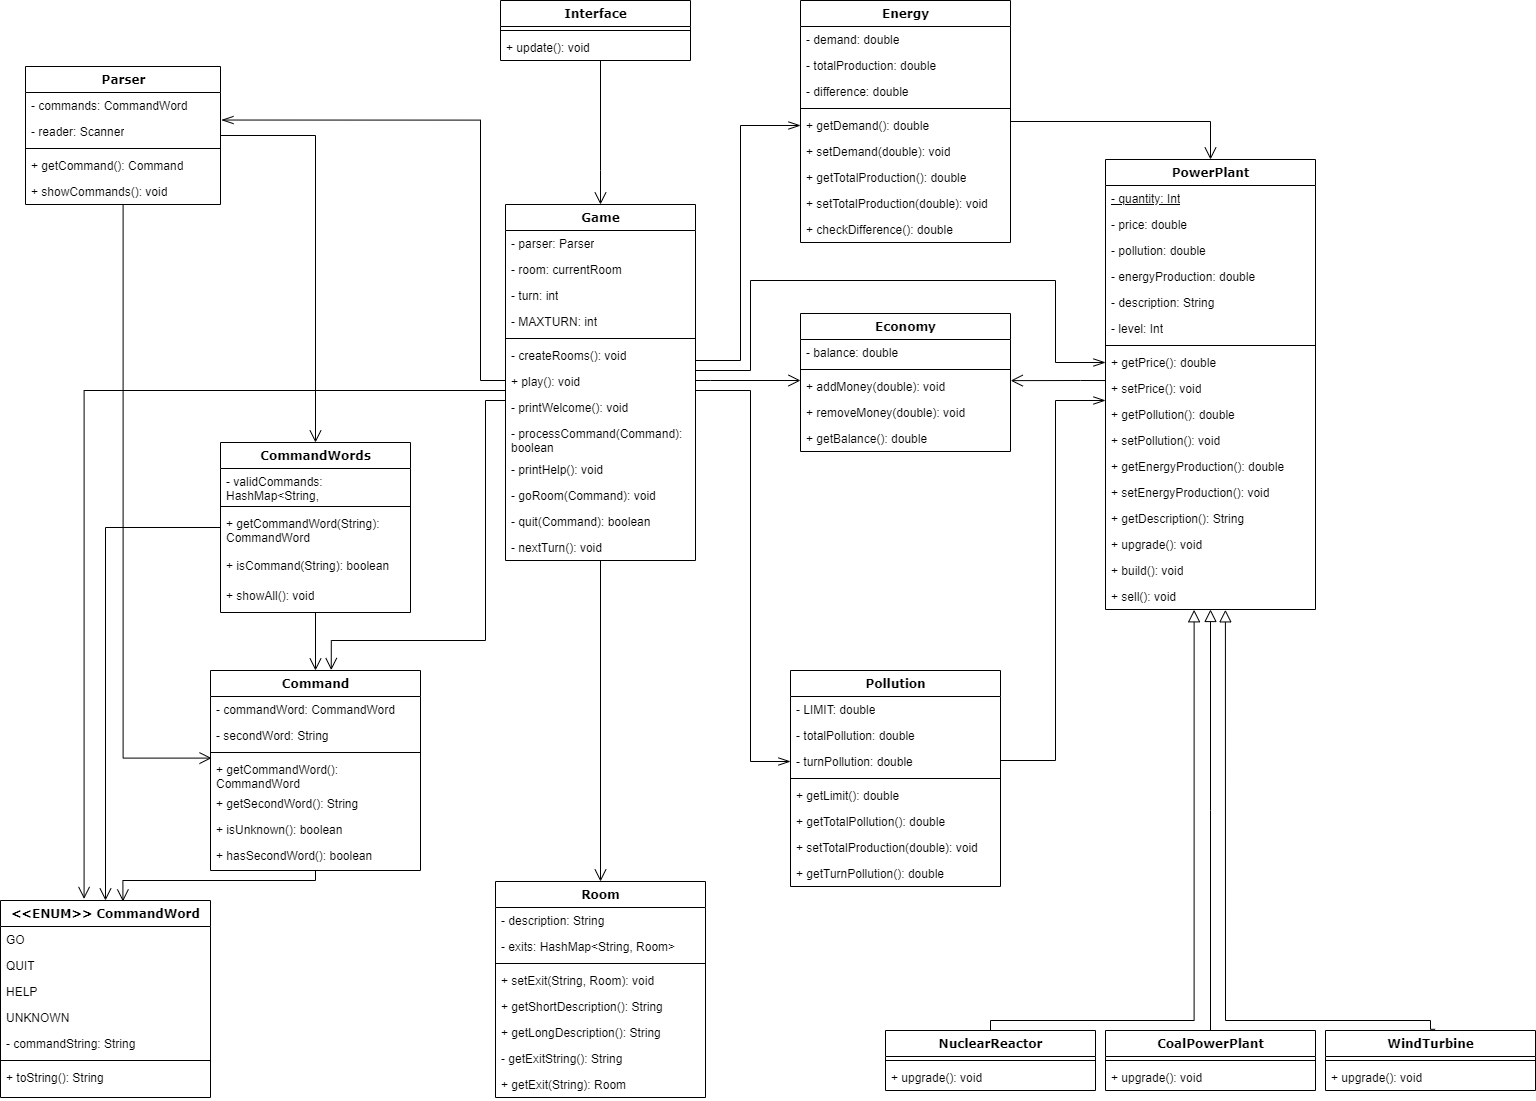
\includegraphics[width=\linewidth]{images/uml_1.png}
	\caption{Der laves et klassediagram, ud fra de overvejelser gruppen har gjort i designfasen.}
	\label{fig:uml}
\end{figure}

\subsection{Implementeringsfasen}
Vi startede ud med at bygge vores spil op efter vores UML diagram.
Undervejs blev vi tvunget til at tænke nærmere over hvordan vores forløb i spillet rent faktisk skulle være, hvordan vores sell og upgrade funktioner skulle fungere. Her har vi også fået tilføjet relevante commandwords, så det er muligt for spilleren at købe og opgradere powerplant, samt at sælge eksisterende power plants. Her har vi også gjort det muligt dels at få vist en komplet liste af alle ejede power plants, men også af en specifik type, for at gøre det muligt for spilleren nemt at vælge lige præcis det powerplant der skal opgraderes eller sælges. I forhold til salg havde vi nogle tanker om at værdien af et powerplant må være lavere end købsprisen hvorfor man ved et salg af et powerplant ikke skal have det fulde beløb tilbage. Vi fik også tænkt nærmere over hvordan at vores energy demand skulle blive øget gennem spillets forløb, sådan at det kom til gradvist at stige mere og mere for hver runde (procentvis forøgelse). Samspillet mellem klasserne er også noget vi har overvejet hvordan vi skulle gøre, og her er det blevet til at det meste er styret centralt fra game klassen.


\bibliographystyle{apacite}
\bibliography{references}
\end{document}